\subsection{\href{https://tensornetwork.org/peps/}{Projected Entangled Pair States}}
Projected entangled pair states (PEPS) - обобщает тензорную сеть tensor train из одномерной сети в сеть на произвольном графе.\\

Тензорная диаграмма для $PEPS$ на конечной квадратной решетке имеет вид:

\begin{figure}[h!tp]
\centering
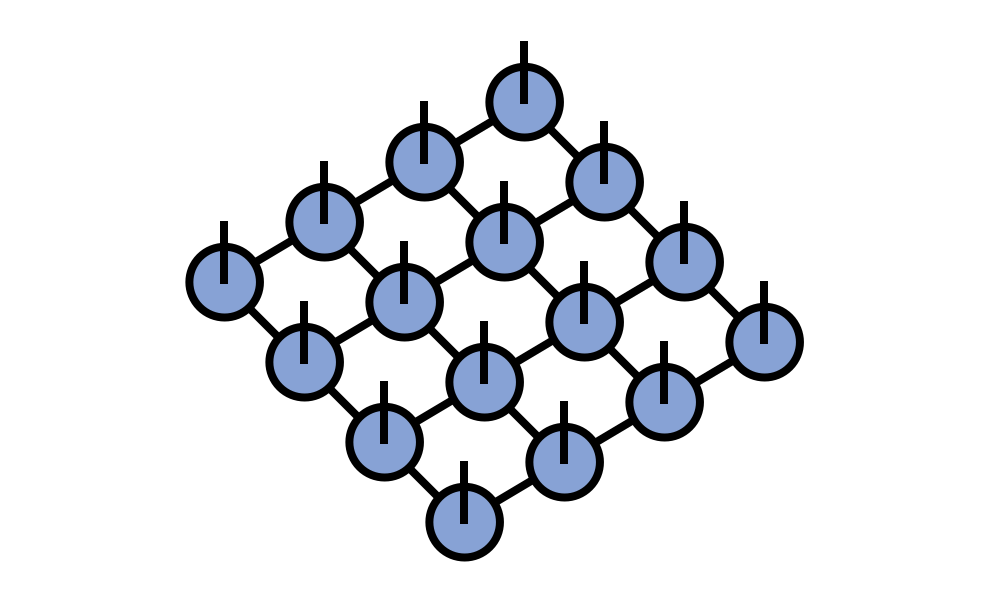
\includegraphics[scale=0.3]{PEPS/PEPS.png}
\caption{Тензорная диаграмма}
\label{fig:PEPSDiag}
\end{figure} 

Название PEPS происходит с той точки зрения на квантовую информацию, согласно которой общие тензорные сети можно рассматривать как максимально коррелированные тензоры в нескольких копиях тензорного индексного пространства, которые затем проецируются в одну копию индексного пространства.